\documentclass[10pt,a4paper,twocolumn]{article}
\usepackage[T1]{fontenc}
\usepackage[utf8]{inputenc}
\usepackage{lmodern}
\usepackage[margin=0.75in,columnsep=0.3in]{geometry}
\usepackage{dblfloatfix}
\usepackage{amsmath,amssymb}
\usepackage{graphicx}
\usepackage{booktabs}
\usepackage{float}
\usepackage[round]{natbib}
\usepackage[hidelinks]{hyperref}
\usepackage{microtype}

\setlength{\parskip}{0.2em}
\raggedbottom

\title{Directional Consistency in Fine-Grained NLI:\\ Baselines for DiCo-NLI (Track 1)}
\author{Muhammad Muneeb Baig, Syed Kamran Ali Shah, Kashaf Ali Haroon\\ MS Data Science, SEECS, NUST\\ CS-878 Deep Learning, Assignment 1}
\date{October 2026}

\begin{document}
\maketitle

\section{Introduction}

Standard NLI accuracy can be achieved using superficial cues. Standard evaluation scores each ordered pair independently, so it cannot show whether a model stays coherent when the pair is reversed. DiCo-NLI (SemEval-2027 Task 2) evaluates both \citep{diconli2026}. We work on Track 1 (English).

\textbf{Black-box view.} The input is an ordered pair of short phrases $(t_1, t_2)$, and the output is one of four labels: EQUIVALENCE (Eq), FORWARD\_\allowbreak{}ENTAILMENT (Fwd), BACKWARD\_\allowbreak{}ENTAILMENT (Bwd) or NEGATIVE\_\allowbreak{}OTHER (Neg). Eq means each phrase implies the other, Fwd that only $t_1 \Rightarrow t_2$, and Bwd that only $t_2 \Rightarrow t_1$. All other relations map to Neg. For example, (\emph{Japanese PM Shinzo Abe}, \emph{Abe}) is Fwd, and the reversed pair is Bwd. A coherent classifier should satisfy $f(t_2, t_1) = \mathrm{rev}(f(t_1, t_2))$, with $\mathrm{rev}(\text{Fwd}) = \text{Bwd}$, $\mathrm{rev}(\text{Bwd}) = \text{Fwd}$ and $\mathrm{rev}(\text{Eq}) = \text{Eq}$. Neg rows appear in only one direction.

\textbf{White-box view.} Fwd and Bwd differ only in direction, so symmetric signals such as word overlap or cosine similarity cannot distinguish them. Equivalence is not similarity: \emph{a sheep} and \emph{an animal} have a lot in common, but the relation is only one-sided. Neg merges several relations, the phrases are very short, and one modifier often determines the label. There is also a length shortcut: the more specific phrase is typically longer, so a model could follow length instead of meaning.

\textbf{Research question and hypotheses.} How far do shallow cues and standard fine-tuned encoders get on DiCo-NLI, and how much of their consistency reflects correct classification? \textbf{H1:} Surface cues (such as length) give non-trivial but modest accuracy and high SoftCons (both metrics are defined in Section~\ref{sec:eval}). \textbf{H2:} Fine-tuned cross-encoders outperform the classical baselines on W-F1 and HardCons. \textbf{H3:} Their remaining errors lie on the Neg boundary rather than on direction.

\section{Related Work}

\citet{gururangan2018annotation} showed that classifiers using only the hypothesis reach about 67\% accuracy on SNLI and 53\% on MultiNLI, well above chance; our length-only and overlap-only probes apply the same idea to phrase pairs. DiCo-NLI is derived from PhrasIS \citep{lopezgazpio2024phrasis}, which has more than 10,000 expert-annotated phrase pairs from captions and headlines; it keeps only reversible relations and maps the rest to Neg \citep{diconli2026}. Language models often fail to retrieve a fact backwards \citep{berglund2024reversal}, but \citet{wu2024reversal} found that BERT did not suffer in this setting, and DiCo-NLI asks the narrower question of whether a predicted relation holds under reversal. The direct predecessor is \citet{apaolaza2026assessing}, who defined soft and hard coherence (the basis of SoftCons and HardCons). On PhrasIS, they evaluated 17 models, attributed the errors of fine-tuned encoders to lexical overlap and prepositions, and cautioned that a model can be consistently incorrect.

\section{Dataset}

The official split is 3,042 training rows (1,760 pair\_ids) and 660 development rows (383 pair\_ids). Because no pair\_id is shared between the splits, a reversed training pair does not leak into development. Seven development rows still have an exact text match in training, which we note as a limitation. Labels are split evenly between Fwd and Bwd (29\% each), with Eq at 26\% and Neg at 16\%. Because Neg is the smallest class, we also report Macro F1. No missing or empty texts or any pairs where $t_1 = t_2$ in train and dev; 116 rows are duplicates of some other $(t_1, t_2)$ pair (one of which has a different label); 18.9\% of rows contain a one-word phrase on at least one side; the longest phrase is 15 words long; all Track 1 pairs are English--English.

\section{Exploratory Data Analysis}

The findings that informed the models are given below; the full plots are in the separate EDA file.

\textbf{Length.} In Fwd rows, $t_1$ averages 3.58 tokens and $t_2$ averages 2.44, and the longer phrase comes first in 77\% of rows. Bwd shows the opposite pattern, while Eq and Neg are both centred on zero (Figure~\ref{fig:eda}, left). Length is a real directional signal, but a surface one, so we test it alone as a shortcut.

\textbf{Overlap and containment.} In 45\% of entailment rows, one phrase's words are fully contained in the other (Figure~\ref{fig:eda}, right). The mean Jaccard is 0.41 for entailment and 0.24 for Eq, because paraphrases use different words. Jaccard is symmetric, so we also add directional containment features.

\textbf{POS.} Adjectives are more common in $t_1$ of Fwd pairs (0.39 per pair vs.\ 0.16 for $t_2$), as are proper nouns and other details that make a phrase more specific. We add POS counts of non-shared words.

\textbf{Similarity and vocabulary.} MiniLM cosine is about 0.74 for entailment, 0.72 for Eq and 0.62 for Neg: it separates related from unrelated pairs but is direction-blind, so the encoders must read both phrases together. 47\% of training word types occur once, and 15.4\% of development tokens are unseen in training, which favours pretrained subword models over TF-IDF.

\begin{figure*}[!t]
  \centering
  \includegraphics[page=2,width=0.49\linewidth]{figures/eda_plots.pdf}\hfill
  \includegraphics[page=5,width=0.49\linewidth]{figures/eda_plots.pdf}
  \caption{Left: signed token-length difference $L(t_1)-L(t_2)$ per label. Right: word-set containment pattern per label (row-normalised). In the plots, FORWARD/BACKWARD/EQUIV/NEG\_OTHER correspond to Fwd/Bwd/Eq/Neg.}
  \label{fig:eda}
\end{figure*}

\section{Feature Engineering}

We construct 26 features for each ordered pair from the EDA: length (token counts and signed difference), symmetric overlap (Jaccard, identical text), directional coverage and containment in both directions, negation and digit mismatch, and spaCy POS counts of non-shared words (noun, proper noun, adjective, verb, preposition, number) on both sides. All features flip under reversal except identical-text and Jaccard. Features are z-scored on the training set.

\section{Baseline Models}

\textbf{Baseline A (classical).} Logistic regression (scikit-learn, $C = 1$) on: length features only; all 26 features; symmetric overlap only, a probe with no notion of direction; TF-IDF unigrams and bigrams, computed separately for each phrase and concatenated in order; and TF-IDF plus features. The floor is a majority-class model.

\textbf{Baseline B (fine-tuned encoders).} \texttt{bert-base-uncased} \citep{devlin2019bert} and \texttt{roberta-base} \citep{liu2019roberta} are fine-tuned end to end as cross-encoders that read $t_1$ and $t_2$ together, with BERT using segment IDs. We use AdamW (lr $3 \times 10^{-5}$, weight decay 0.01), batch size 16, linear warm-up and six epochs, and keep the final epoch according to a rule fixed in advance. Each model is trained with three seeds (13, 42, 87) on an Apple M4 GPU. An early BERT run dropped \texttt{token\_type\_ids}; after the fix, the setup was frozen.

\section{Evaluation Setup}
\label{sec:eval}

We use the organisers' scorer on the 660 development rows, of which 554 are reversible, giving $M = 277$ pairs. Weighted F1 weights per-class F1 by class support; Macro F1 gives each class a weight of 1. For pair $i$ with predictions $\hat{y}_{i,1}, \hat{y}_{i,2}$ and gold labels $y_{i,1}, y_{i,2}$:
\begin{align}
\text{SoftCons} &= \frac{1}{M}\sum_{i=1}^{M} \mathbf{1}\left[\hat{y}_{i,1} \neq \text{Neg} \wedge \hat{y}_{i,2} = \mathrm{rev}(\hat{y}_{i,1})\right] \\
\text{HardCons} &= \frac{1}{M}\sum_{i=1}^{M} \mathbf{1}\left[\hat{y}_{i,1} = y_{i,1} \wedge \hat{y}_{i,2} = y_{i,2}\right]
\end{align}
HardCons requires a model to be both consistent and correct; SoftCons only checks consistency. Because HardCons also requires correctness, $\text{HardCons} \leq \text{SoftCons}$.

\section{Results}

Table~\ref{tab:main} gives the main picture. LR on only four length features reaches 0.464 W-F1 and an almost perfect 0.989 SoftCons. The symmetric-overlap probe is blind to direction and manages only 0.368 SoftCons. Directional features raise W-F1 to 0.593, and adding TF-IDF gives the best classical model (0.620). Both encoders clearly improve on this, with RoBERTa reaching a mean of $0.765 \pm 0.002$ W-F1; it is also much more consistent across seeds than BERT. The largest per-class gain is on Eq (F1 0.515 $\to$ 0.725 for RoBERTa): as the EDA showed, paraphrases share few words, so they need the lexical knowledge that pretraining brings. Neg is the worst class for all models. For Fwd, the extra proper nouns, adjectives and nouns on the $t_1$ side push towards the label ($+0.59$, $+0.49$, $+0.53$), while the extra nouns on the $t_2$ side push away ($-0.72$); for Neg, both containment directions are negative ($-0.65$, $-0.46$). The sign of the length features is not interpreted because these are collinear (len\_diff $-0.53$ vs.\ char\_diff $+0.47$ for Fwd). Note also that the encoders have lower SoftCons than the classical feature models (0.774--0.804 vs.\ 0.856--0.877) but higher HardCons. Figure~\ref{fig:curves} shows the training runs: loss decreases steadily, and the final-epoch rule costs little, since development W-F1 levels off after three or four epochs.

\begin{table*}[!t]
\centering
\small
\resizebox{\textwidth}{!}{%
\begin{tabular}{lccccc}
\toprule
Model & W-F1 & SoftCons & HardCons & Macro-F1 & Acc. \\
\midrule
Majority class & 0.129 & 0.000 & 0.000 & 0.112 & 0.288 \\
LR (length only) & 0.464 & \textbf{0.989} & 0.628 & 0.408 & 0.532 \\
LR (symmetric overlap only) & 0.324 & 0.368 & 0.188 & 0.291 & 0.370 \\
LR (engineered features) & 0.593 & 0.877 & 0.653 & 0.558 & 0.602 \\
TF-IDF + LR & 0.484 & 0.877 & 0.542 & 0.452 & 0.500 \\
TF-IDF + features + LR & 0.620 & 0.856 & 0.661 & 0.588 & 0.626 \\
\midrule
BERT-base (3 seeds) & 0.705 $\pm$ 0.023 & 0.774 $\pm$ 0.016 & 0.693 $\pm$ 0.021 & 0.680 $\pm$ 0.024 & 0.707 $\pm$ 0.020 \\
RoBERTa-base (3 seeds) & \textbf{0.765 $\pm$ 0.002} & 0.804 $\pm$ 0.011 & \textbf{0.739 $\pm$ 0.006} & \textbf{0.742 $\pm$ 0.002} & \textbf{0.762 $\pm$ 0.004} \\
\bottomrule
\end{tabular}}
\caption{Development-set results with the official scorer. W-F1, SoftCons and HardCons are the official metrics.}
\label{tab:main}
\end{table*}

\begin{figure*}[!t]
  \centering
  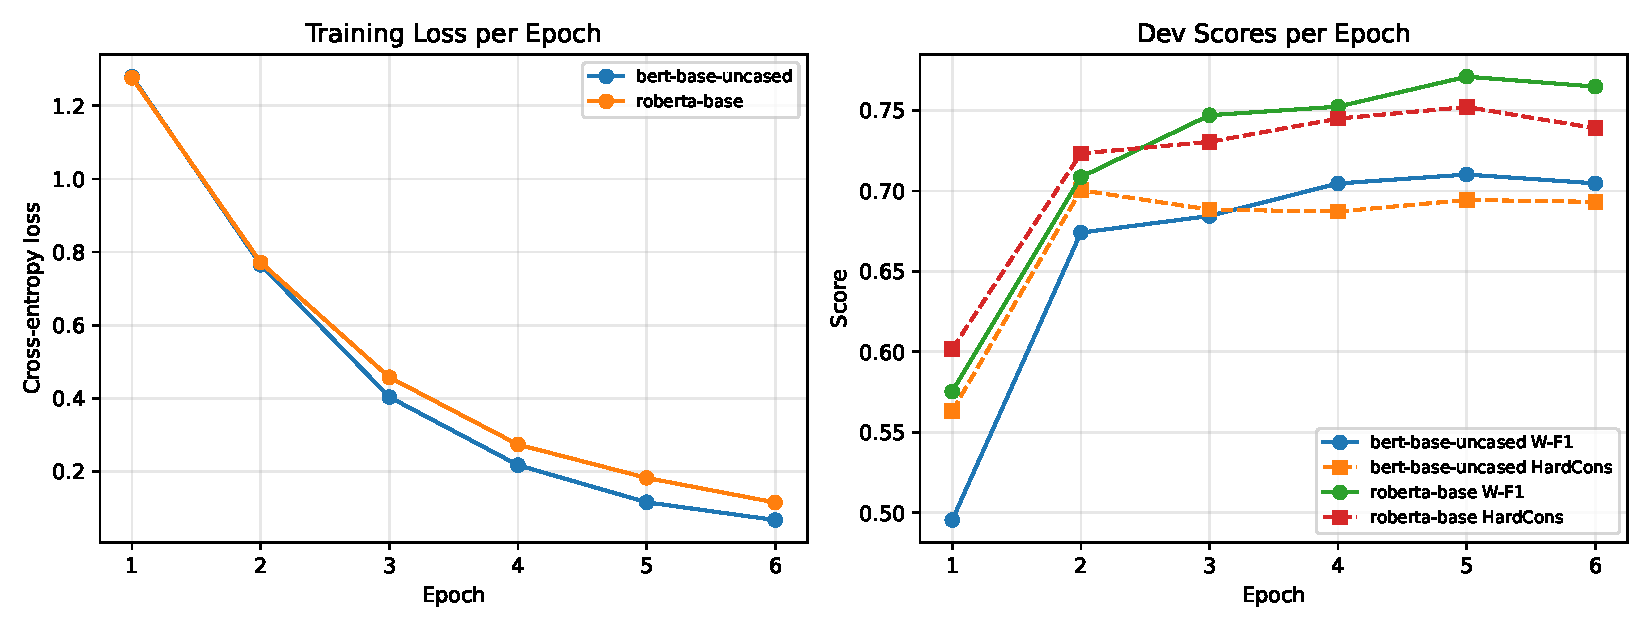
\includegraphics[width=0.75\textwidth]{figures/training_curves.pdf}
  \caption{Training loss (left) and development W-F1 and HardCons (right) per epoch, averaged over three seeds. Not used for model selection.}
  \label{fig:curves}
\end{figure*}

\section{Error Analysis}

Table~\ref{tab:errors} breaks down the 277 reversible pairs by joint outcome (seed-42 encoders vs.\ the best classical model).

Much of the classical model's consistency is consistent wrongness (54 pairs). RoBERTa has only 16 such pairs and confuses Fwd with Bwd only twice in each direction, compared with 7 and 9 times for the classical model. However, its errors sit in the Neg row and column, as with the classical model (Figure~\ref{fig:cm}). Its main problem is predicting Neg for only one orientation (42 pairs), which is what lowers its SoftCons.

\emph{Same-sex marriage} / \emph{gay marriage} is Eq, but the length-only model, the best classical model and RoBERTa all predict Fwd/Bwd: consistent, and wrong. \emph{A monochrome photograph} / \emph{a black and white photo} splits the models: TF-IDF plus features gives Bwd/Fwd, BERT gives Eq/Neg, and only RoBERTa gets Eq both ways. RoBERTa's largest error group (69 rows) is rejecting near-paraphrases and related pairs as Neg, such as \emph{martial arts clubs} / \emph{martial arts schools}. As in \citet{apaolaza2026assessing}, prepositions also cause errors. Finally, BERT without segment IDs assigned the same label to both orientations in 119 of 190 entailment pairs, and in none once they were restored.

\begin{table}[!htb]
\centering
\resizebox{\columnwidth}{!}{%
\begin{tabular}{lccc}
\toprule
Outcome & TF-IDF + feats & BERT & RoBERTa \\
\midrule
Both directions correct & 183 & 186 & \textbf{204} \\
Consistent but wrong & 54 & 28 & 16 \\
Same entailment label both ways & 4 & 4 & 0 \\
Neg in one direction only & 35 & 47 & 42 \\
Other inconsistency & 1 & 12 & 15 \\
\bottomrule
\end{tabular}}
\caption{Outcomes for the 277 reversible development pairs (encoders: seed 42).}
\label{tab:errors}
\end{table}

\begin{figure*}[!t]
  \centering
  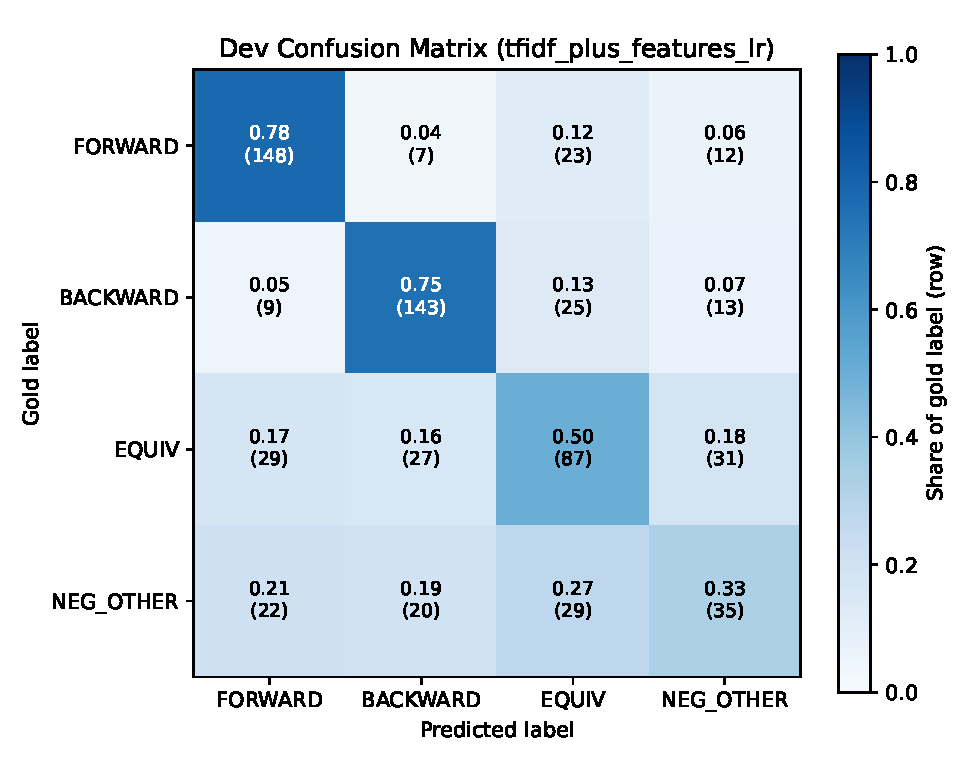
\includegraphics[width=0.49\linewidth]{figures/confusion_tfidf.pdf}\hfill
  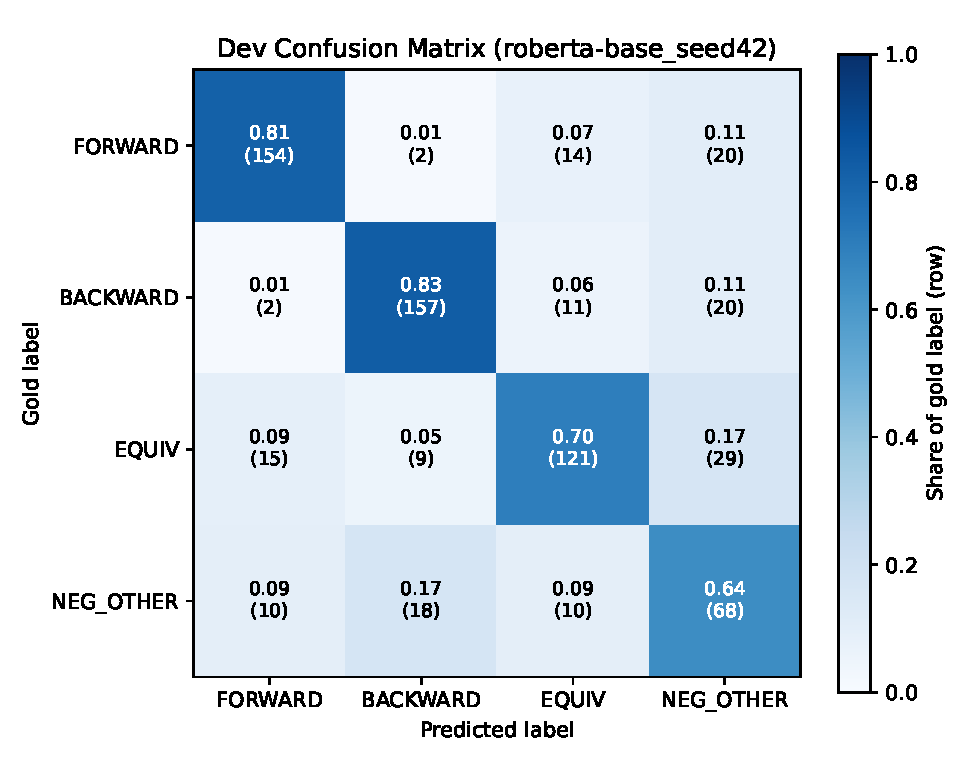
\includegraphics[width=0.49\linewidth]{figures/confusion_roberta.pdf}
  \caption{Row-normalised development confusion matrices: TF-IDF + features LR (left) and RoBERTa-base, seed 42 (right). FORWARD/BACKWARD/EQUIV/NEG\_OTHER correspond to Fwd/Bwd/Eq/Neg.}
  \label{fig:cm}
\end{figure*}

\section{Discussion}

All three hypotheses are supported. Length alone gave near-perfect consistency with mediocre classification (H1); RoBERTa clearly beat the classical baselines on W-F1 and HardCons (H2); and the encoders handled direction with little difficulty, leaving the Neg boundary as the main failure (H3). The clearest lesson is that SoftCons is not a measure of correctness: the most consistent model in the study is the one that only looks at phrase length.

\textbf{Limitations.} We evaluate on the public development split (7 rows overlap with training) and did no hyperparameter search. MPS training is not fully deterministic (up to 0.03 W-F1 between identical runs), and we use only three seeds. Error categories come from heuristic rules, and some gold labels are debatable (\emph{Australian senator} / \emph{Australian lawmaker} is Neg). DeBERTa-v3 was dropped after NaN losses on MPS.

\section{Next Steps}

The one-sided Neg errors call for predicting both orientations jointly, or for training with a reversal-consistency loss that enforces $f(t_2, t_1) = \mathrm{rev}(f(t_1, t_2))$. We will also try class weighting for Neg, run DeBERTa-v3 on CUDA, and make a blind test submission.

\small
\bibliographystyle{plainnat}
\bibliography{references}

\end{document}
